\chapter{Architecture du Système}
\label{chap:Architecture}

L'architecture du système représente l'organisation et la structure du logiciel, des composants et de leurs interactions. Ce chapitre présente l'architecture du système pour la plateforme de mise en relation entre agences de location de voitures et particuliers, en utilisant PostgreSQL avec PostGIS, Django, et DTL (Django Template Language). 

\section{Vue d'ensemble de l'architecture}
L'architecture de ce système est basée sur une architecture cliente-serveur avec une séparation claire entre le backend, le frontend et la base de données. Le système utilise les technologies suivantes :

\begin{itemize}
    \item \textbf{Backend} : Django est utilisé comme framework de développement web. Il est responsable de la logique métier, de la gestion des utilisateurs, des réservations, des paiements, et des interactions avec la base de données.
    \item \textbf{Frontend} : DTL (Django Template Language) est utilisé pour générer dynamiquement les pages web côté client, avec un design réactif pour une expérience utilisateur optimale sur différents appareils.
    \item \textbf{Base de données} : PostgreSQL avec l'extension PostGIS pour la gestion des données géospatiales (localisation des agences, etc.).
\end{itemize}

\section{Composants Principaux de l'Architecture}
L'architecture du système repose sur plusieurs composants clés :
\begin{itemize}
    \item \textbf{Client (Frontend)} : Les utilisateurs interagissent avec l'interface utilisateur via des pages web générées dynamiquement. Les pages sont responsables de l'affichage des informations et de la collecte des données de l'utilisateur (réservations, paiements, etc.).
    \item \textbf{Serveur (Backend)} : Django gère la logique de l'application, y compris la gestion des utilisateurs, la gestion des véhicules et des agences, les réservations, et la communication avec la base de données.
    \item \textbf{Base de données (PostgreSQL + PostGIS)} : PostgreSQL sert de système de gestion de base de données relationnelle, tandis que PostGIS permet de gérer les données géospatiales. Cela est particulièrement utile pour la gestion des emplacements des véhicules et des réservations géolocalisées.
    \item \textbf{API Restful (Django REST Framework)} : Une API est mise en place pour permettre la communication entre le frontend et le backend. Cette API est utilisée pour récupérer des données sur les véhicules, les réservations, et autres informations nécessaires.
\end{itemize}

\section{Diagrammes de l'Architecture}
Voici un diagramme simplifié qui montre l'interaction entre les différents composants du système.

\begin{figure}[h!]
    \centering
    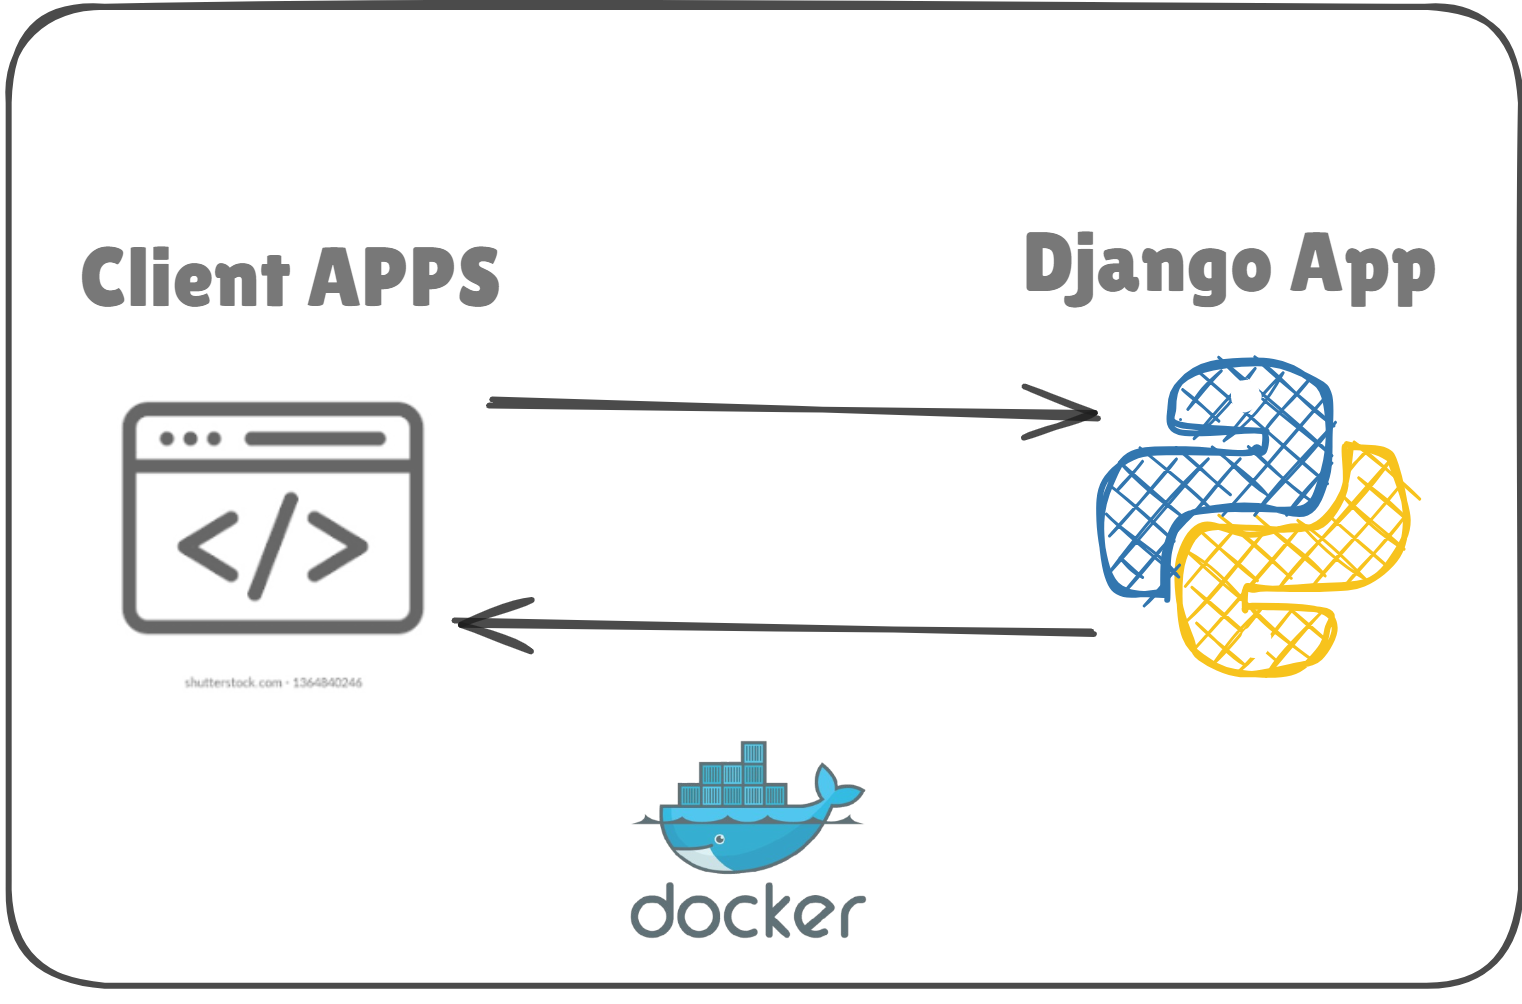
\includegraphics[width=0.8\textwidth]{images/architecureg.png}
    \caption{Diagramme de l'Architecture du Système}
    \label{fig:system_architecture}
\end{figure}

\subsection{Backend avec Django}
Le backend est construit avec le framework Django, qui fournit un ensemble de fonctionnalités pour gérer les utilisateurs, la logique métier et la base de données. Django repose sur un modèle MVC (Modèle-Vue-Contrôleur), où :

\begin{itemize}
    \item \textbf{Modèle (Model)} : Définit la structure de la base de données, les relations entre les entités et les règles métiers.
    \item \textbf{Vue (View)} : Gère la logique de présentation et rend les données sous forme de pages HTML dynamiques.
    \item \textbf{Contrôleur (Controller)} : Django agit principalement comme contrôleur en acheminant les demandes des utilisateurs et en renvoyant des réponses appropriées.
\end{itemize}

Django est également couplé avec Django REST Framework (DRF) pour permettre la création d'APIs Restful pour les interactions entre le frontend et le backend.

\subsection{Gestion des données géospatiales avec PostGIS}
L'extension PostGIS de PostgreSQL est utilisée pour gérer les données géospatiales. Elle permet de stocker et de traiter les informations géographiques, comme les coordonnées GPS des véhicules et des agences. Cette capacité géospatiale est particulièrement utile pour des fonctionnalités comme :
\begin{itemize}
    \item La recherche de véhicules disponibles dans une zone géographique donnée.
    \item L'affichage de la localisation des véhicules sur une carte.
    \item La gestion des réservations en fonction de la proximité géographique entre l'utilisateur et les véhicules disponibles.
\end{itemize}

\begin{figure}[h!]
    \centering
    \includegraphics[width=0.8\textwidth]{database_schema.png}
    \caption{Schéma de la Base de Données avec PostGIS}
    \label{fig:database_schema}
\end{figure}

Le schéma de la base de données inclut des tables pour les utilisateurs, les agences, les véhicules, les réservations et les paiements. Chaque véhicule est associé à une géolocalisation, ce qui permet de les retrouver facilement dans une zone géographique donnée.

\section{Flux de Données}
Lorsqu'un utilisateur souhaite réserver un véhicule, voici le flux de données typique :
\begin{enumerate}
    \item L'utilisateur effectue une recherche sur la plateforme avec des filtres géographiques et de disponibilité.
    \item Le frontend envoie une requête au backend via l'API Restful de Django.
    \item Le backend interroge la base de données PostgreSQL pour trouver les véhicules disponibles dans la zone géographique demandée.
    \item La réponse est envoyée au frontend, qui affiche les véhicules disponibles sur la carte.
    \item Une fois la réservation confirmée, les détails sont enregistrés dans la base de données, y compris la géolocalisation du véhicule réservé.
\end{enumerate}

\section{Implémentation des Fonctionnalités Clés}

\subsection{Système de Transfert}

Le système de transfert est une fonctionnalité majeure de la plateforme qui permet aux utilisateurs de réserver des véhicules avec chauffeur. Cette section détaille son architecture et son implémentation.

\subsection{Modèles de Données}
Le système de transfert repose sur deux modèles principaux :

\begin{itemize}
    \item \textbf{TransferVehicle} :
    \begin{itemize}
        \item Types de véhicules : voiture, van, minibus, bus
        \item Informations sur le véhicule (marque, modèle, capacité)
        \item Tarification horaire et durée minimale
        \item Informations sur le chauffeur (nom, téléphone, expérience, langues)
    \end{itemize}
    
    \item \textbf{TransferBooking} :
    \begin{itemize}
        \item Gestion des points de ramassage et de dépôt (PostGIS)
        \item Horaires et durée estimée
        \item Nombre de passagers
        \item Statut de la réservation (en attente, confirmé, en cours, terminé, annulé)
    \end{itemize}
\end{itemize}

\subsection{Fonctionnalités Géospatiales}
L'intégration de PostGIS permet une gestion avancée des données géographiques :

\begin{itemize}
    \item Stockage des coordonnées en format WGS84 (SRID 4326)
    \item Transformation automatique des coordonnées Web Mercator
    \item Calcul des distances et des itinéraires optimaux
    \item Visualisation sur carte interactive
\end{itemize}

\subsection{Gestion des Réservations}
Le processus de réservation inclut :

\begin{itemize}
    \item \textbf{Recherche} :
    \begin{itemize}
        \item Filtrage par type de véhicule
        \item Disponibilité selon la date et l'heure
        \item Capacité passagers
        \item Localisation géographique
    \end{itemize}
    
    \item \textbf{Réservation} :
    \begin{itemize}
        \item Validation de la disponibilité
        \item Calcul automatique du prix total
        \item Gestion des conflits de réservation
        \item Notifications automatiques
    \end{itemize}
\end{itemize}

\subsection{Sécurité et Validation}
Plusieurs niveaux de sécurité sont implémentés :

\begin{itemize}
    \item Validation des données de réservation
    \item Vérification des permissions d'agence
    \item Protection CSRF pour les formulaires
    \item Journalisation des actions sensibles
\end{itemize}

\begin{figure}[h!]
    \centering
    \includegraphics[width=0.8\textwidth]{docs/transfer_class_diagram.puml}
    \caption{Diagramme de classes du système de transfert}
    \label{fig:transfer_class_diagram}
\end{figure}

\subsection{API et Interfaces}
Le système expose plusieurs points d'accès :

\begin{itemize}
    \item API REST pour la gestion des véhicules
    \item Endpoints pour la recherche géospatiale
    \item Interface de réservation intuitive
    \item Tableau de bord administratif
\end{itemize}

\section{Sécurité et Performance}

\subsection{Mesures de Sécurité}
La sécurité du système est assurée par plusieurs mécanismes :

\begin{itemize}
    \item \textbf{Authentification et Autorisation} :
    \begin{itemize}
        \item Système d'authentification Django avec tokens
        \item Gestion fine des permissions par rôle (admin, agent, utilisateur)
        \item Protection contre les attaques CSRF
    \end{itemize}
    
    \item \textbf{Sécurité des Données} :
    \begin{itemize}
        \item Chiffrement des mots de passe avec l'algorithme PBKDF2
        \item Protection des données sensibles (informations de paiement)
        \item Validation des entrées utilisateur
    \end{itemize}
    
    \item \textbf{Sécurité des Sessions} :
    \begin{itemize}
        \item Gestion sécurisée des sessions Django
        \item Délai d'expiration des sessions
        \item Protection contre le détournement de session
    \end{itemize}
\end{itemize}

\subsection{Optimisation des Performances}
Pour garantir une expérience utilisateur optimale, plusieurs stratégies d'optimisation ont été mises en place :

\begin{itemize}
    \item \textbf{Cache} :
    \begin{itemize}
        \item Mise en cache des requêtes fréquentes
        \item Utilisation du cache de template Django
        \item Cache des données géospatiales
    \end{itemize}
    
    \item \textbf{Optimisation des Requêtes} :
    \begin{itemize}
        \item Utilisation des select\_related() et prefetch\_related()
        \item Index sur les champs fréquemment utilisés
        \item Pagination des résultats de recherche
    \end{itemize}
    
    \item \textbf{Gestion des Ressources} :
    \begin{itemize}
        \item Compression des fichiers statiques
        \item Optimisation des images
        \item Utilisation de Docker pour la gestion des ressources
    \end{itemize}
\end{itemize}

\subsection{Monitoring et Maintenance}
Le système inclut des fonctionnalités de surveillance :

\begin{itemize}
    \item Journalisation des événements importants
    \item Surveillance des performances avec Django Debug Toolbar
    \item Analyse des erreurs et exceptions
    \item Métriques de performance PostgreSQL
\end{itemize}

\section{Conclusion}
L'architecture du système est conçue pour garantir une haute performance, une évolutivité et une sécurité tout en répondant aux exigences de géolocalisation. L'utilisation de PostgreSQL avec PostGIS permet une gestion optimale des données géospatiales, tandis que Django offre une plateforme robuste pour le développement de l'application web. L'API Restful facilite l'interaction entre le frontend et le backend, assurant ainsi une expérience utilisateur fluide.

\section{Patterns de Conception et Modélisation}

\subsection{Patterns de Conception Utilisés}
L'application implémente plusieurs patterns de conception pour assurer sa maintenabilité et son évolutivité :

\begin{itemize}
    \item \textbf{Pattern MVC (MVT)} :
    \begin{itemize}
        \item \textit{Models} : Gestion des données et logique métier
        \item \textit{Views} : Logique de présentation et API
        \item \textit{Templates} : Interface utilisateur
    \end{itemize}
    
    \item \textbf{Factory Pattern} :
    \begin{itemize}
        \item Création des objets de réservation
        \item Instanciation des véhicules
        \item Génération des notifications
    \end{itemize}
    
    \item \textbf{Observer Pattern} :
    \begin{itemize}
        \item Notifications des changements de statut
        \item Mise à jour des disponibilités
        \item Événements de réservation
    \end{itemize}
    
    \item \textbf{Strategy Pattern} :
    \begin{itemize}
        \item Calcul des prix
        \item Validation des réservations
        \item Gestion des paiements
    \end{itemize}
\end{itemize}

\subsection{Diagrammes de Classes}
Le système est structuré autour des classes principales suivantes :

\begin{figure}[h!]
    \centering
    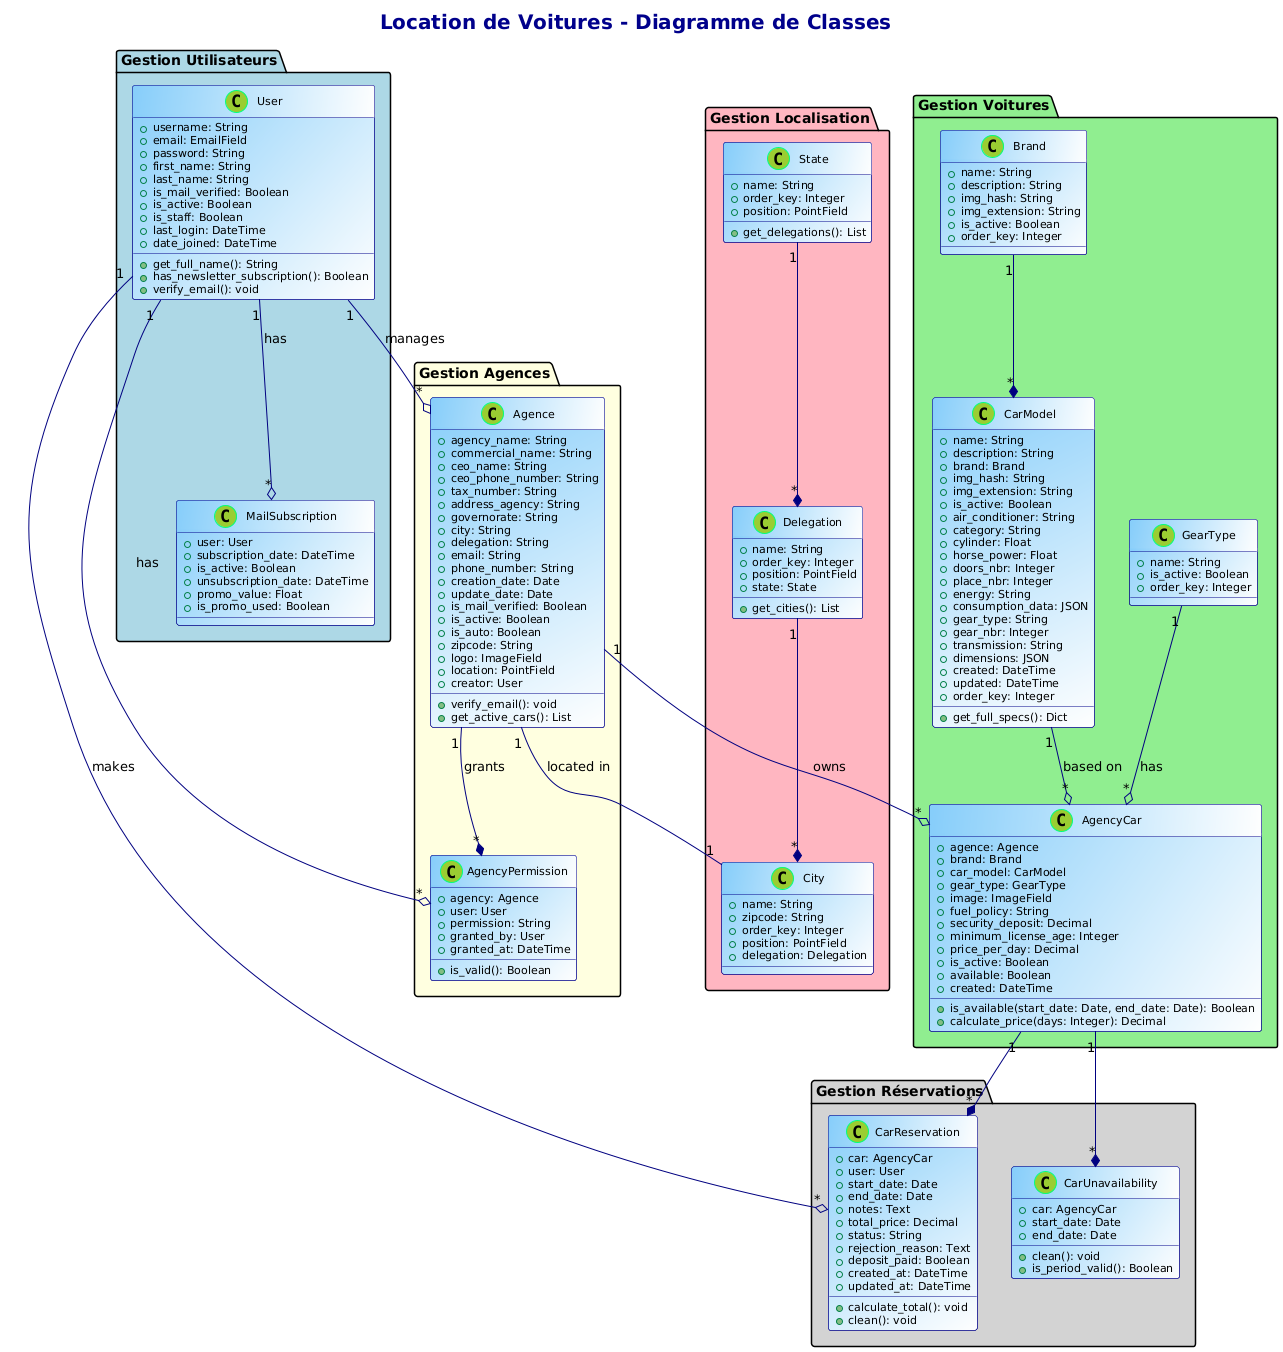
\includegraphics[width=1\textwidth]{docs/rapport/class.png}
    \caption{Diagramme de classes principal}
    \label{fig:class_diagram}
\end{figure}

\begin{itemize}
    \item \textbf{Modèles de Base} :
    \begin{itemize}
        \item \texttt{User} : Gestion des utilisateurs
        \item \texttt{Agency} : Information des agences
        \item \texttt{Vehicle} : Données des véhicules
        \item \texttt{Reservation} : Gestion des réservations
    \end{itemize}
    
    \item \textbf{Modèles Géospatiaux} :
    \begin{itemize}
        \item \texttt{Location} : Points géographiques
        \item \texttt{Route} : Trajets et itinéraires
        \item \texttt{Area} : Zones de service
    \end{itemize}
\end{itemize}

\subsection{Diagrammes de Séquence}
Les principales interactions du système sont modélisées comme suit :

\begin{figure}[h!]
    \centering
    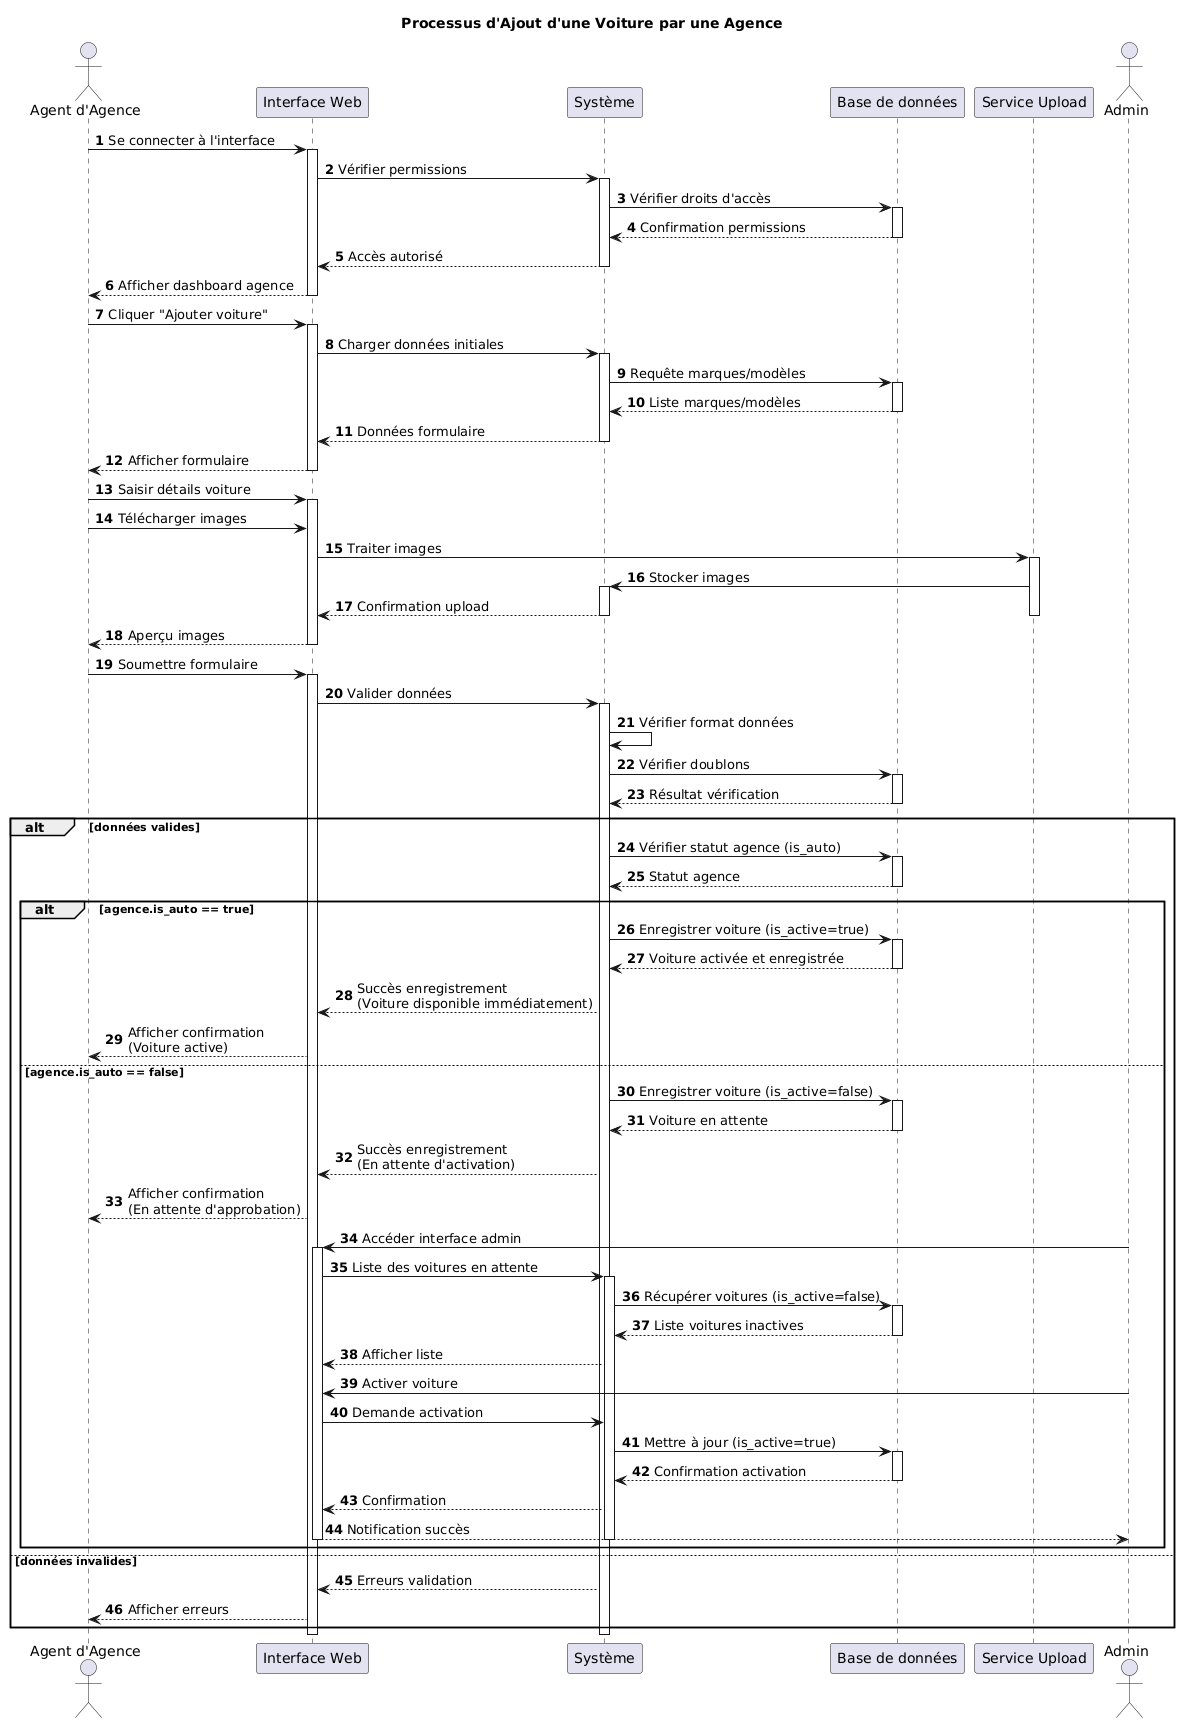
\includegraphics[width=1\textwidth]{docs/rapport/sequence.png}
    \caption{Diagramme de séquence - Processus de réservation}
    \label{fig:sequence_diagram}
\end{figure}

Le diagramme illustre :
\begin{itemize}
    \item Recherche de véhicules disponibles
    \item Vérification des disponibilités
    \item Processus de réservation
    \item Notification des parties
\end{itemize}

\subsection{Diagrammes de Cas d'Utilisation}
Les principaux cas d'utilisation sont :

\begin{figure}[h!]
    \centering
    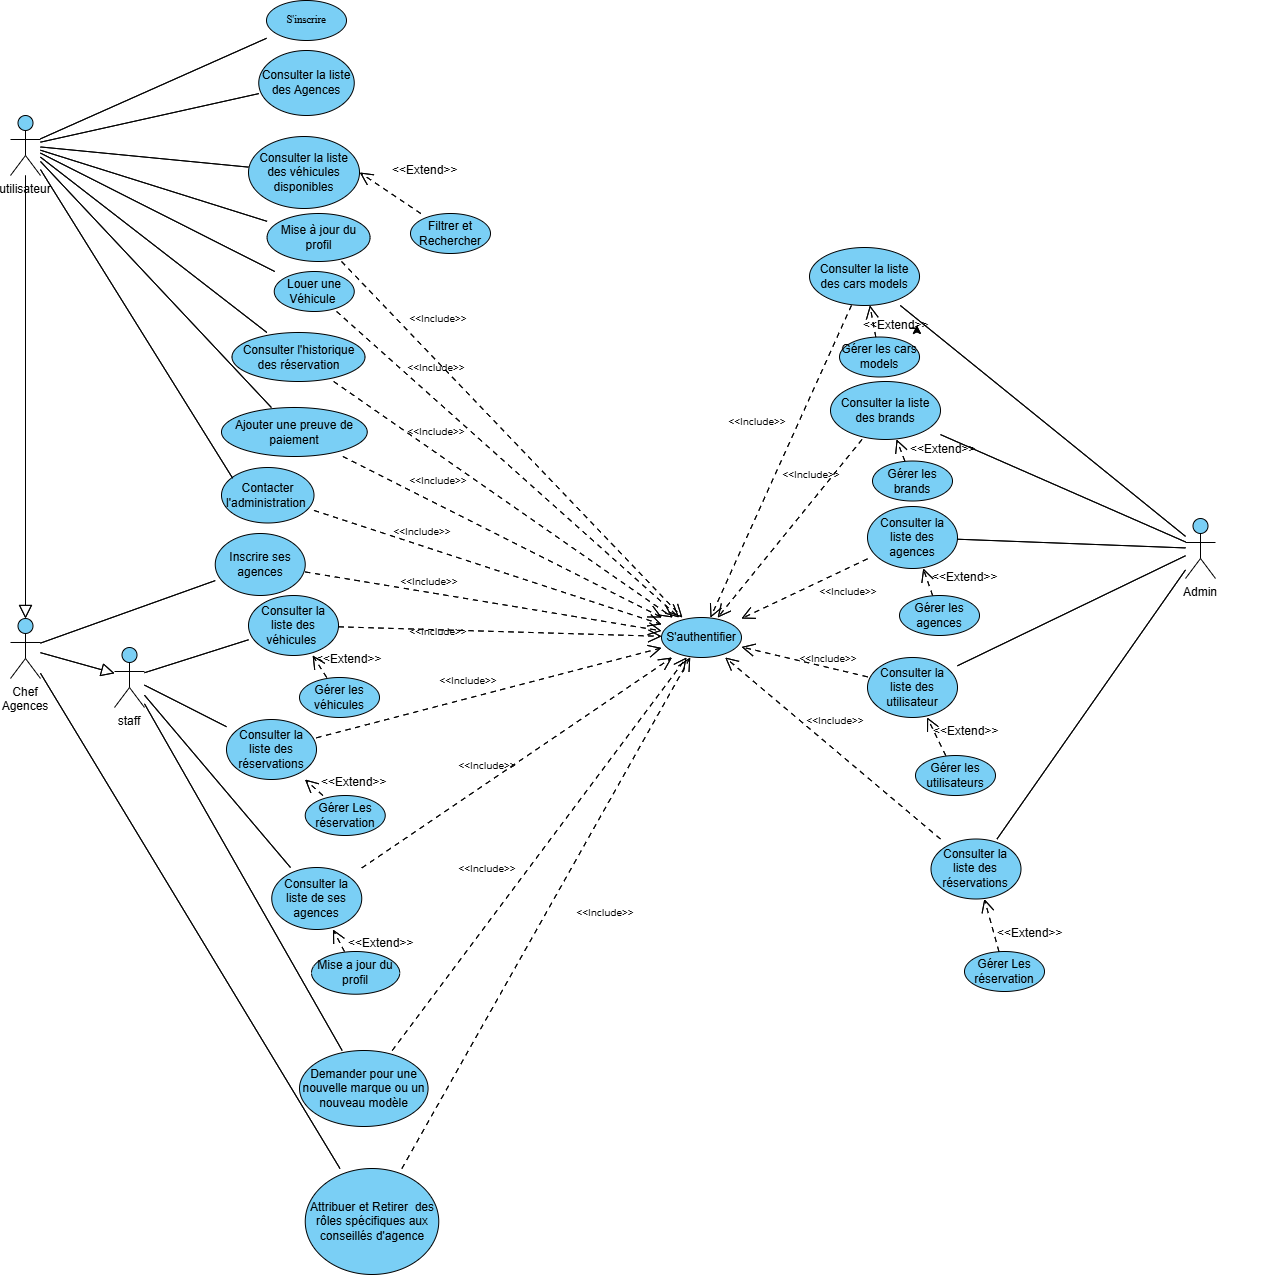
\includegraphics[width=1\textwidth]{docs/rapport/Use Case Pfe (3).png}
    \caption{Diagramme des cas d'utilisation}
    \label{fig:usecase_diagram}
\end{figure}

\begin{itemize}
    \item \textbf{Gestion des Utilisateurs} :
    \begin{itemize}
        \item Inscription et authentification
        \item Gestion du profil
        \item Gestion des préférences
    \end{itemize}
    
    \item \textbf{Gestion des Réservations} :
    \begin{itemize}
        \item Recherche de véhicules
        \item Création de réservations
        \item Suivi des réservations
        \item Gestion des paiements
    \end{itemize}
    
    \item \textbf{Administration} :
    \begin{itemize}
        \item Gestion des agences
        \item Validation des comptes
        \item Suivi des statistiques
    \end{itemize}
\end{itemize}

\section{Architecture Détaillée des Composants}

\subsection{Couche Présentation}
L'interface utilisateur est construite avec :

\begin{itemize}
    \item \textbf{Templates Django} :
    \begin{itemize}
        \item Structure modulaire
        \item Héritage de templates
        \item Internationalisation intégrée
    \end{itemize}
    
    \item \textbf{JavaScript} :
    \begin{itemize}
        \item Interactions dynamiques
        \item Validation côté client
        \item Gestion des cartes
    \end{itemize}
    
    \item \textbf{CSS/Bootstrap} :
    \begin{itemize}
        \item Design responsive
        \item Thème personnalisé
        \item Composants réutilisables
    \end{itemize}
\end{itemize}

\subsection{Couche Métier}
La logique métier est organisée en services :

\begin{itemize}
    \item \textbf{Services de Réservation} :
    \begin{itemize}
        \item Validation des disponibilités
        \item Gestion des conflits
        \item Calcul des tarifs
    \end{itemize}
    
    \item \textbf{Services Géospatiaux} :
    \begin{itemize}
        \item Recherche par proximité
        \item Calcul d'itinéraires
        \item Optimisation des zones
    \end{itemize}
    
    \item \textbf{Services de Notification} :
    \begin{itemize}
        \item Emails transactionnels
        \item Notifications temps réel
        \item Rappels automatiques
    \end{itemize}
\end{itemize}

\subsection{Couche Données}
La persistance des données est assurée par :

\begin{itemize}
    \item \textbf{PostgreSQL} :
    \begin{itemize}
        \item Schéma relationnel optimisé
        \item Contraintes d'intégrité
        \item Transactions ACID
    \end{itemize}
    
    \item \textbf{PostGIS} :
    \begin{itemize}
        \item Index spatiaux
        \item Requêtes géographiques
        \item Optimisation spatiale
    \end{itemize}
    
    \item \textbf{Cache} :
    \begin{itemize}
        \item Cache de session
        \item Cache de requête
        \item Cache de template
    \end{itemize}
\end{itemize}

\section{Documentation des API}

\subsection{API de Gestion des Véhicules}
Les endpoints principaux pour la gestion des véhicules :

\begin{table}[h]
\centering
\begin{tabular}{|p{3cm}|p{2cm}|p{8cm}|}
\hline
\textbf{Endpoint} & \textbf{Méthode} & \textbf{Description} \\
\hline
\texttt{/api/vehicles/} & GET & Liste des véhicules disponibles avec filtres \\
\hline
\texttt{/api/vehicles/\{id\}} & GET & Détails d'un véhicule spécifique \\
\hline
\texttt{/api/vehicles/search/} & POST & Recherche avancée avec critères géographiques \\
\hline
\texttt{/api/vehicles/availability/} & GET & Vérification des disponibilités \\
\hline
\end{tabular}
\caption{API de gestion des véhicules}
\label{tab:vehicle_api}
\end{table}

\subsection{API de Réservation}
Endpoints pour la gestion des réservations :

\begin{table}[h]
\centering
\begin{tabular}{|p{3cm}|p{2cm}|p{8cm}|}
\hline
\textbf{Endpoint} & \textbf{Méthode} & \textbf{Description} \\
\hline
\texttt{/api/bookings/} & POST & Création d'une nouvelle réservation \\
\hline
\texttt{/api/bookings/\{id\}} & GET & Détails d'une réservation \\
\hline
\texttt{/api/bookings/status/} & PUT & Mise à jour du statut \\
\hline
\texttt{/api/bookings/cancel/} & POST & Annulation d'une réservation \\
\hline
\end{tabular}
\caption{API de gestion des réservations}
\label{tab:booking_api}
\end{table}

\subsection{API Géospatiale}
Services géospatiaux exposés :

\begin{table}[h]
\centering
\begin{tabular}{|p{3cm}|p{2cm}|p{8cm}|}
\hline
\textbf{Endpoint} & \textbf{Méthode} & \textbf{Description} \\
\hline
\texttt{/api/geo/search/} & GET & Recherche par zone géographique \\
\hline
\texttt{/api/geo/routes/} & POST & Calcul d'itinéraires \\
\hline
\texttt{/api/geo/areas/} & GET & Zones de service disponibles \\
\hline
\end{tabular}
\caption{API géospatiale}
\label{tab:geo_api}
\end{table}

\subsection{Format des Requêtes}
Exemple de requête pour la recherche de véhicules :

\begin{verbatim}
POST /api/vehicles/search/
{
    "location": {
        "lat": 36.8065,
        "lng": 10.1815
    },
    "radius": 5000,
    "startDate": "2025-05-01",
    "endDate": "2025-05-03",
    "vehicle_type": "car",
    "capacity": 4
}
\end{verbatim}

\subsection{Format des Réponses}
Exemple de réponse pour une recherche de véhicules :

\begin{verbatim}
{
    "status": "success",
    "count": 2,
    "results": [
        {
            "id": 1,
            "brand": "Toyota",
            "model": "Corolla",
            "year": 2024,
            "price_per_day": 150.00,
            "location": {
                "type": "Point",
                "coordinates": [10.1815, 36.8065]
            },
            "distance": 1200,
            "availability": true
        },
        {
            "id": 2,
            ...
        }
    ]
}
\end{verbatim}

\subsection{Gestion des Erreurs}
Format standardisé des erreurs :

\begin{verbatim}
{
    "status": "error",
    "code": "INVALID_DATES",
    "message": "Les dates sélectionnées ne sont pas valides",
    "details": {
        "startDate": "La date de début doit être postérieure à aujourd'hui",
        "endDate": "La date de fin doit être postérieure à la date de début"
    }
}
\end{verbatim}

\subsection{Sécurité des API}
Mesures de sécurité implémentées :

\begin{itemize}
    \item \textbf{Authentification} :
    \begin{itemize}
        \item JWT (JSON Web Tokens)
        \item Expiration des tokens
        \item Rotation des clés
    \end{itemize}
    
    \item \textbf{Autorisations} :
    \begin{itemize}
        \item RBAC (Role-Based Access Control)
        \item Scopes d'API
        \item Quotas par utilisateur
    \end{itemize}
    
    \item \textbf{Protection} :
    \begin{itemize}
        \item Rate limiting
        \item Validation des entrées
        \item CORS configuré
    \end{itemize}
\end{itemize}

\subsection{Versioning des API}
Stratégie de versioning :

\begin{itemize}
    \item Version dans l'URL (\texttt{/api/v1/})
    \item Gestion de la rétrocompatibilité
    \item Documentation des changements
    \item Période de dépréciation
\end{itemize}

\subsection{Monitoring des API}
Outils de surveillance :

\begin{itemize}
    \item \textbf{Métriques} :
    \begin{itemize}
        \item Temps de réponse
        \item Taux d'erreur
        \item Utilisation des ressources
    \end{itemize}
    
    \item \textbf{Alertes} :
    \begin{itemize}
        \item Seuils de performance
        \item Erreurs critiques
        \item Disponibilité
    \end{itemize}
    
    \item \textbf{Logs} :
    \begin{itemize}
        \item Requêtes/réponses
        \item Erreurs détaillées
        \item Audit des accès
    \end{itemize}
\end{itemize}

